\documentclass[11pt]{article}
\usepackage[a4paper,margin=25mm]{geometry}
\usepackage{amsmath,amssymb,amsthm,mathtools}
\usepackage{booktabs,array,longtable}
\usepackage[dvipsnames]{xcolor}
\usepackage{hyperref,fancyhdr,graphicx}
\hypersetup{hypertexnames=false,colorlinks=true,linkcolor=MidnightBlue,urlcolor=MidnightBlue,citecolor=MidnightBlue,
pdftitle={A sharper packing criterion for self-pinned distances}}
\setlength{\parindent}{0pt}\setlength{\parskip}{5pt}
\setlength{\emergencystretch}{2em}\setlength{\headheight}{14pt}
\pagestyle{fancy}\fancyhf{}\fancyhead[L]{\small Self-pinned distance sets}
\fancyhead[R]{\small Refined sufficient condition}\fancyfoot[C]{\thepage}
\newtheorem{theorem}{Theorem}[section]
\newtheorem{proposition}[theorem]{Proposition}
\newtheorem{lemma}[theorem]{Lemma}
\theoremstyle{definition}\newtheorem{remark}[theorem]{Remark}
\newcommand{\R}{\mathbb R}\newcommand{\HH}{\dim_{\mathrm H}}\newcommand{\PP}{\dim_{\mathrm P}}
\newcommand{\supp}{\operatorname{supp}}\newcommand{\dist}{\operatorname{dist}}
\newcommand{\dd}{\,d}\newcommand{\norm}[1]{\left\|#1\right\|}\newcommand{\eps}{\varepsilon}

\begin{document}
\begin{titlepage}
\vspace*{18mm}
{\large\color{MidnightBlue} RESEARCH MANUSCRIPT}\par
\vspace{8mm}
{\Huge\bfseries A sharper packing criterion}\par
\vspace{5mm}
{\LARGE for self-pinned distance sets}\par
\vspace{12mm}
30 September 2026
\vspace{12mm}

This note weakens the packing restriction in the 19 September manuscript.
The scale-selection argument splits according to the location of a profile minimum
above the mandatory midpoint. An affine-envelope estimate handles the remaining case.
Both analytic branches and the Borel-set reduction are included.

\textbf{What is proved here.} Subject to the cited established analytic theorems,
the manuscript gives a mathematical proof of the revised sufficient condition.
It also proves a stronger conditional-energy convergence criterion.

\textbf{What remains unresolved.} No weakest possible condition, optimality theorem,
or unrestricted improvement of the five-quarters threshold is proved.
The proof has received separate internal mathematical checks, but no external referee
review and no complete Lean verification. A comparator check of a conditional branch
combination would not certify either analytic branch or this new theorem.

\vfill
The prior theorem and the prior Lean target are preserved. This note is a new
research result, not a declaration that an open formalization is finished.
\end{titlepage}
\tableofcontents
\clearpage
\section{Statement and scope}
For a Borel set \(E\subset\R^2\), put \(d=\HH E\), \(D=\PP E\), and
\(\Delta_y(E)=\{|x-y|:x\in E\}\). All distances are Euclidean and
\(|\cdot|\) denotes one-dimensional Lebesgue measure. Set
$$
 d_A=\frac{4+\sqrt{10}}6\approx1.193712943,\qquad
 d_B=\frac{47+\sqrt{649}}{60}\approx1.207924640.
$$
For \(1<d\le5/4\), define
\begin{equation}\label{fprof:curve}
 B_{\rm new}(d)=\begin{cases}
 2d-1,&1<d\le d_A,\\[4pt]
 \dfrac{d(8d-7)}{d+1},&d_A<d\le d_B,\\[8pt]
 3d-\dfrac{13}{6},&d_B<d\le\dfrac{11}{9},\\[8pt]
 \dfrac{7d-6+\sqrt{49d^2-96d+56}}4,&\dfrac{11}{9}<d\le\dfrac54.
 \end{cases}
\end{equation}
\begin{theorem}[Refined sufficient condition]\label{target:main}
If \(E\subset\R^2\) is Borel, \(1<\HH E\le5/4\), and
$$
 \PP E<B_{\rm new}(\HH E),
$$
then \(|\Delta_y(E)|>0\) for some \(y\in E\).
\end{theorem}
The inequality is strict. The proof produces separated compact source and pin
subsets of \(E\); in fact the selected source probability has absolutely continuous
pinned distance laws for almost every pin under the selected pin probability.
Distance images of Borel sets are analytic and Lebesgue measurable.

For example, this covers
$$
 d=\frac{31}{25}=1.24,\qquad D=\frac{77}{50}=1.54.
$$
The quoted previous cutoff at this dimension was \(1.506696\ldots\), whereas
\(B_{\rm new}(1.24)=1.546869432\ldots\).
The two analytic costs and the strict margin are
$$
 E(d,D)=\frac{1009}{4650},\qquad L(d,D)=\frac{609}{2600},\qquad
 (d-1)-\max\{E(d,D),L(d,D)\}=\frac3{520}>0.
$$
This slack permits the use of Frostman exponents strictly below the Hausdorff
dimension and a covering exponent strictly above the packing dimension.

\begin{figure}[ht]
\centering
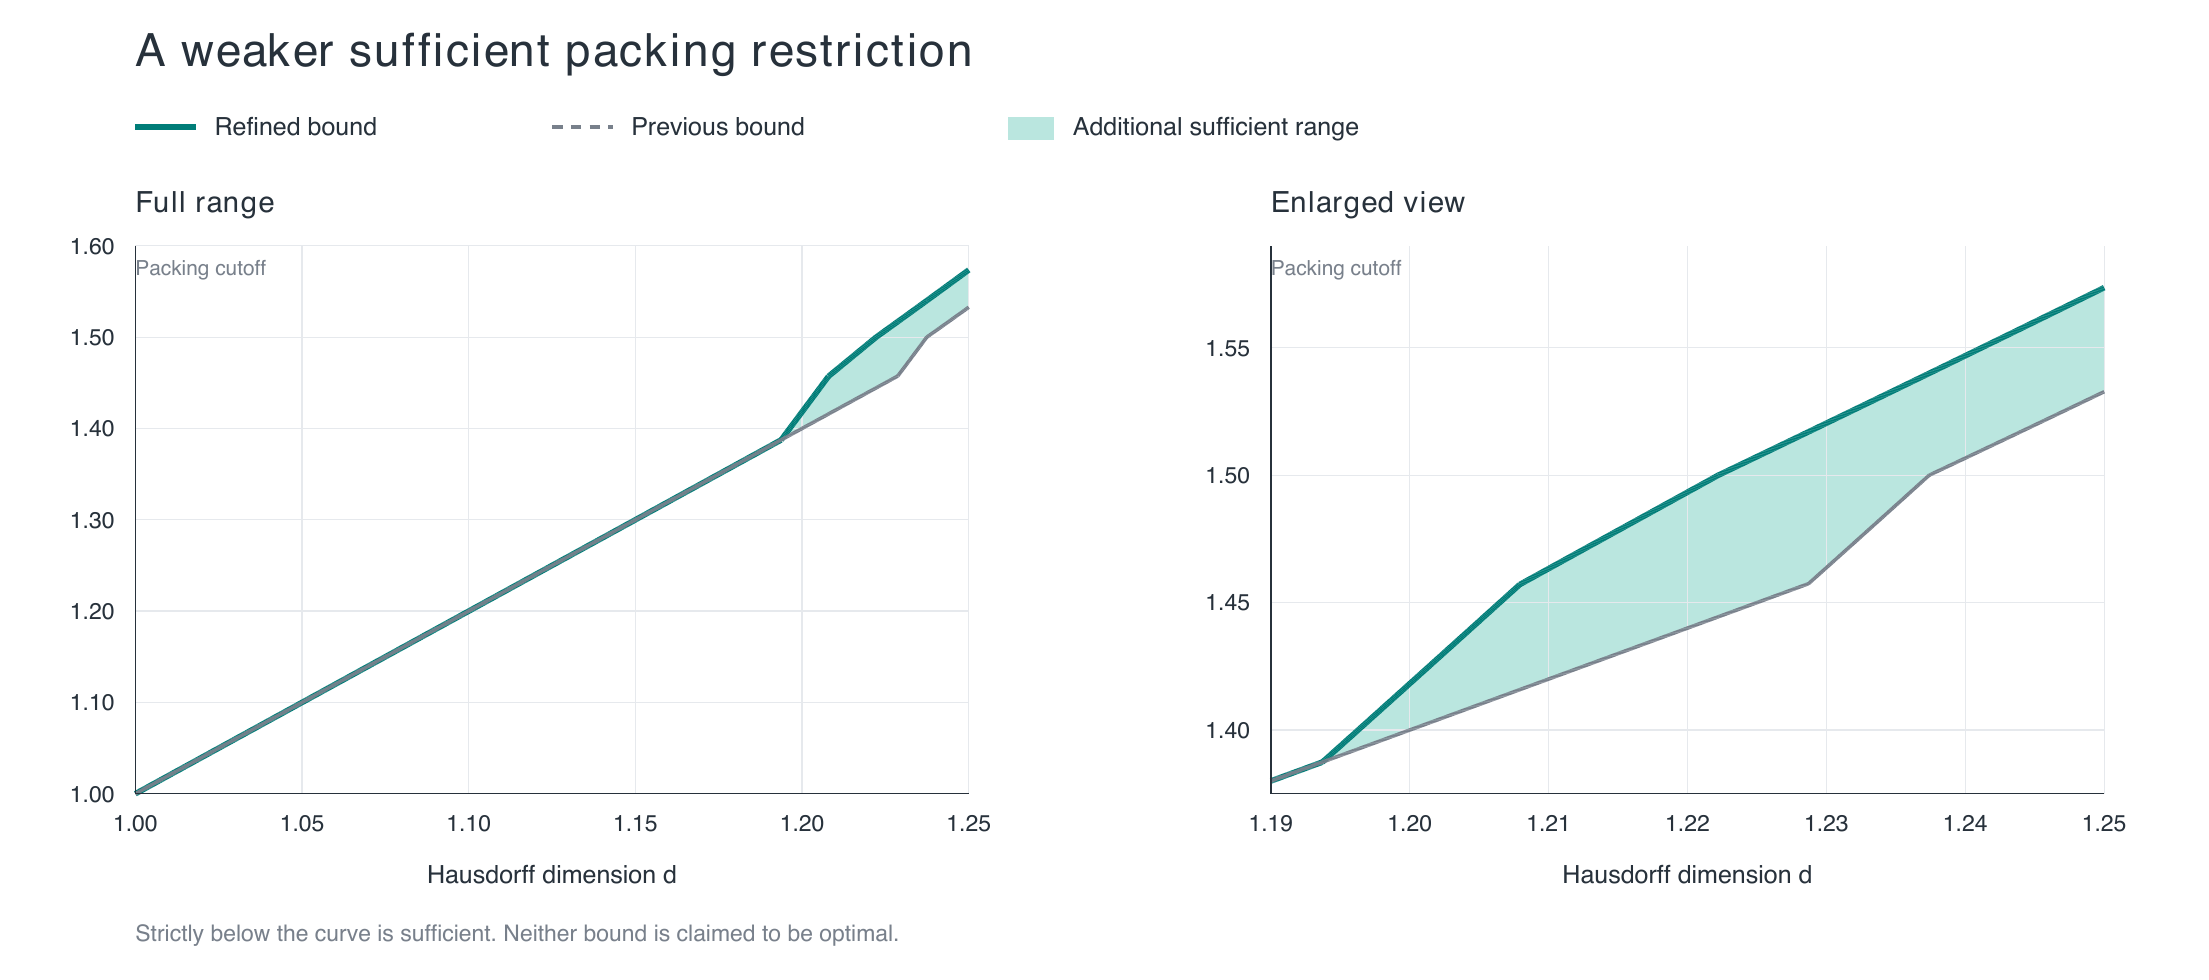
\includegraphics[width=\textwidth]{../figures/packing-refinement.png}
\caption{The refined sufficient bound compared with the previous one. The right
panel enlarges the interval where the new bound gives a strict gain.
Neither curve is asserted to be a necessary condition.}
\end{figure}

\subsection{Definitions and established inputs}
A probability \(\mu\) is \(s\)-Frostman if
\(\mu(B(x,r))\le C r^s\) for \(0<r\le1\). Write
$$
 I_a(\mu)=\iint |x-x'|^{-a}\dd\mu(x)\dd\mu(x').
$$
An \(s\)-Frostman probability of bounded support has finite \(a\)-energy
whenever \(0<a<s\), by summing spatial annuli.
The external inputs are as follows.
\begin{enumerate}
\item Frostman's lemma for Borel subsets of Euclidean space, and the
countable bounded-cover characterization of packing dimension using upper box dimension.
Closures preserve bounded upper box dimension; positive-mass compact restrictions
are available by inner regularity.
\item Orponen's averaged radial-projection integrability \cite{orponen}, in the form
of GIOW Theorem 3.7 or Keleti--Shmerkin Theorem 3.11. For separated compact
Frostman probabilities of exponents greater than one, radial projections have
\(L^q\) densities for some \(q>1\), with integrable \(q\)-th powers of their norms.
\item Plancherel, the Riesz energy identity, polar coordinates and their projection
consequences, with Fourier normalization
\(\widehat f(\xi)=\int e^{-2\pi i x\cdot\xi}f(x)\,dx\).
\item Keleti--Shmerkin Lemma 3.4 and Corollary 3.5 \cite{ks}, used only for finite
terminal-cube restrictions, not to extract an infinite regular subset.
\item The elementary packet localization of GIOW Section 3 \cite{giow},
Liu's cap reconstruction (Lemma 4.2 of \cite{liu2026}), and the pinned quadratic
identity \cite{liuidentity}. The variable-chain inflation multiplier is derived below.
\end{enumerate}
All constants may depend on the fixed compact supports, positive source-pin
separation and chosen auxiliary parameters. They are uniform in frequency,
regularized component, cube and cap. The notation \(\operatorname{RapDec}(R)\)
means a quantity bounded by \(C_MR^{-M}\) for every fixed \(M>0\), uniformly
in those indices. Summing polynomially many such errors preserves this property.
The constants in losses \(R^{C_Kh}\) are independent of the regularization block
size \(T\); fixed annular ratios depending on \(T\) only change multiplicative constants.

\clearpage
\section{Coherent positive linearizations and a conditional convergence theorem}
\label{sec:coherenttree}

This section proves the original branch of the bound, rather than assuming Proposition E.6 from the longer report. It uses positive affine approximations to distance and a summable first-norm comparison.

\subsection{Angular regularity with a single exceptional set}

\begin{lemma}[Coupled-angle projection comparison]\label{lem:coherentangular}
Let \(0<\gamma<1/2\), and let \(\lambda\) be a probability supported in \(B(0,Cr)\), \(0<r\leq1\), with \(I_{1+2\gamma}(\lambda)<\infty\). For almost every \(\theta\in S^1\), let \(F(\theta)\in L^2(\R)\) be the density of \((\pi_\theta)_*\lambda\), where \(\pi_\theta(x)=x\cdot\theta\). There is a nonnegative function \(G\) with
$$
\|G\|_{L^2(S^1)}^2\leq C_\gamma r^{2\gamma}I_{1+2\gamma}(\lambda)
$$
such that, outside one angular null set, every pair satisfies
$$
\|F(\theta)-F(\phi)\|_{L^2(\R)}
\leq C_\gamma d(\theta,\phi)^\gamma\bigl(G(\theta)+G(\phi)\bigr),
$$
where \(d\) is circular arclength distance. In addition,
$$
\int_{S^1}\sup_{|v|\leq Cr^2}
\|F(\theta)(\cdot-v)-F(\theta)\|_2^2d\theta
\leq C_\gamma r^{4\gamma}I_{1+2\gamma}(\lambda).
$$
\end{lemma}
\begin{proof}
We first prove the Hilbert-valued angular Sobolev estimate
\begin{equation}\label{eq:coherentangularsobolev}
\|F\|_{H^\gamma(S^1;L^2(\R))}^2
\leq C_\gamma r^{2\gamma}I_{1+2\gamma}(\lambda).
\end{equation}
The projection-energy identity gives the projected densities and their joint second integrability, since finite \((1+2\gamma)\)-energy implies finite first energy on the bounded support. Fourier transform in the scalar projection variable. The transformed function is
$$
f_\tau(\theta)=\widehat\lambda(\tau\theta).
$$
Its angular derivative is a linear combination, with bounded angular coefficients, of \(\tau\widehat{x_k\lambda}(\tau\theta)\), \(k=1,2\). The Riesz energy identity for these signed measures gives
$$
\int_{\R^2}|\widehat{x_k\lambda}(\xi)|^2|\xi|^{2\gamma-1}d\xi
\leq C_\gamma r^2I_{1+2\gamma}(\lambda).
$$
Indeed the spatial double integral has the factor \(x_kx'_k\), whose absolute value is at most \(Cr^2\). Its absolute energy is finite, so approximation justifies the signed Fourier identity.

Angular Sobolev interpolation, or directly Holder on angular Fourier coefficients, gives
$$
\|f_\tau\|_{H^\gamma}^2
\leq\|f_\tau\|_2^{2(1-\gamma)}\|f_\tau\|_{H^1}^{2\gamma}.
$$
On \(|\tau|\geq1/r\), introduce the canceling weights
$$
A_\tau=|\tau|^{2\gamma}\|f_\tau\|_2^2,
\qquad
B_\tau=|\tau|^{-2(1-\gamma)}\|f_\tau\|_{H^1}^2.
$$
Polar coordinates and the preceding signed-energy estimate show
$$
\int_{|\tau|\geq1/r}A_\tau d\tau\leq C_\gamma I_{1+2\gamma}(\lambda),
\qquad
\int_{|\tau|\geq1/r}B_\tau d\tau\leq C_\gamma r^2I_{1+2\gamma}(\lambda).
$$
For the undifferentiated part of \(B_\tau\), use \(|\tau|^{-2}\leq r^2\); its derivative part has exactly the energy weight after the factor \(\tau^2\) is inserted. Holder in \(\tau\) now bounds the integral of \(\|f_\tau\|_{H^\gamma}^2\) by \(C_\gamma r^{2\gamma}I_{1+2\gamma}(\lambda)\) on this region. When \(|\tau|\leq1/r\), both \(f_\tau\) and its angular derivative are bounded uniformly, so the contribution is at most \(C/r\). This is absorbed because
$$
I_{1+2\gamma}(\lambda)\geq (Cr)^{-1-2\gamma}.
$$
Plancherel in the scalar variable proves \eqref{eq:coherentangularsobolev}.

Choose a measurable Hilbert-valued representative and define
$$
G(\theta)^2
=\int_{S^1}\frac{\|F(\theta)-F(z)\|_2^2}{d(\theta,z)^{1+2\gamma}}dz.
$$
The angular Slobodeckij identity gives \(\|G\|_2^2\leq C_\gamma\|F\|_{H^\gamma}^2\). For completeness, expand in angular Fourier coefficients: translation invariance makes each nonzero coefficient contribute its squared Hilbert norm times
$$
\int_{-\pi}^{\pi}\frac{|e^{ikh}-1|^2}{|h|^{1+2\gamma}}dh
\asymp_\gamma |k|^{2\gamma}.
$$
Tonelli and Parseval prove the assertion also for Hilbert-valued functions.

Remove the null set where \(G\) is infinite, where \(F\) is undefined, or where it does not represent the projected density. Given two remaining angles at distance \(\delta>0\), take an arc \(J\) of length comparable to \(\delta\) containing both, with every point of \(J\) within \(C\delta\) of each endpoint. Average the triangle inequality through \(z\in J\). Cauchy--Schwarz gives
$$
\begin{aligned}
\|F(\theta)-F(\phi)\|_2
&\leq |J|^{-1/2}
\left[\left(\int_J\|F(\theta)-F(z)\|_2^2dz\right)^{1/2}
+\left(\int_J\|F(\phi)-F(z)\|_2^2dz\right)^{1/2}\right]\\
&\leq C_\gamma\delta^\gamma\bigl(G(\theta)+G(\phi)\bigr).
\end{aligned}
$$
For large \(\delta\), the whole circle serves as \(J\); the diagonal case is immediate. This proves a single-null-set, all-pairs estimate, which can be evaluated on correlated angular laws.

Finally Plancherel bounds the translation expression, before angular integration, by
$$
Cr^{4\gamma}\int_\R |\tau|^{2\gamma}|\widehat\lambda(\tau\theta)|^2d\tau.
$$
Here the supremum over \(|v|\leq Cr^2\) was bounded inside the Fourier integral, using \(|e^{-2\pi i\tau v}-1|^2\leq C_\gamma|\tau v|^{2\gamma}\). Polar coordinates give the required translation bound.
\end{proof}

\subsection{Consecutive positive linearizations}

Let \(\mu,\nu\) be compact probabilities with positively separated supports, satisfying Frostman bounds with exponents \(s,t>1\). Choose
$$
0<\gamma<\min\left(\frac12,\frac{s-1}{2}\right).
$$
For a positive-mass dyadic source square \(Q\), write \(p_Q=\mu(Q)\), \(\mu_Q=p_Q^{-1}\mu|_Q\). Orponen's theorem, in the GIOW Theorem 3.7 form stated in the preliminaries \cite{orponen,giow}, supplies \(q>1\) and
$$
(\Theta_x)_*\nu=\rho_xd\sigma,\qquad
\Theta_x(y)=\frac{x-y}{|x-y|},\qquad
B=\int\|\rho_x\|_q^q d\mu(x)<\infty,
$$
where \(\sigma\) is normalized arclength. The hypotheses follow by choosing a common Frostman exponent between one and \(\min(s,t)\). In every node choose \(x_Q\in Q\cap\supp\mu\) at which the density exists and
$$
F_Q:=\|\rho_{x_Q}\|_q^q\leq\frac2{p_Q}\int_Q\|\rho_x\|_q^q d\mu(x).
$$
There are countably many nodes, and these choices give
$$
\sum_{Q\text{ at level }n}p_QF_Q\leq2B
\quad\text{at every level.}
$$
Define the affine approximation
$$
L_Q(x,y)=\Theta_{x_Q}(y)\cdot(x-y).
$$
At level \(n\), push the original positive pair probability by \((x,y)\mapsto(y,L_{Q_n(x)}(x,y))\). It has a nonnegative density \(f_n\) relative to \(\nu(dy)dt\). To see this, each \(\mu_Q\) has finite first energy and therefore second-integrable projected densities for almost every angle. Its chosen center's angular pin law is absolutely continuous, so the assertion holds for almost every pin, simultaneously at all countably many nodes. The conditional densities can be chosen jointly measurably. Each \(f_n\) has mass one, and Taylor's theorem gives
$$
|L_{Q_n(x)}(x,y)-|x-y||\leq C2^{-2n}
$$
uniformly, once the squares are smaller than the fixed separation.

\begin{proposition}[Coherent first-norm comparison]\label{prop:coherentcomparison}
For \(r=2^{-n}\) sufficiently small and every \(A\geq1\),
\begin{equation}\label{eq:coherentcomparison}
\|f_{n+1}-f_n\|_{L^1(\nu\times dt)}
\leq C\left[
A r^{1+4\gamma}\sum_{Q\text{ at level }n+1}p_QI_{1+2\gamma}(\mu_Q)
\right]^{1/2}+CB A^{1-q}.
\end{equation}
Constants depend on the fixed support geometry and separation, the exponents and Frostman bounds, but not on \(n,A\).
\end{proposition}
\begin{proof}
Let \(Q\) be a child of \(P\), and apply both affine maps to the same conditional source \(\mu_Q\). Set \(b=x_Q\), and recenter this source at \(b\). Put \(\theta=\Theta_{x_P}(y)\), \(\phi=\Theta_b(y)\). Their separation is \(O(r)\), and
$$
L_P(x,y)=\theta\cdot(x-b)+\theta\cdot(b-y),\qquad
L_Q(x,y)=\phi\cdot(x-b)+|b-y|.
$$
The constants differ quadratically:
$$
|\theta\cdot(b-y)-|b-y||
=|b-y|\,|\theta\cdot\phi-1|\leq Cr^2.
$$
Recentring is essential here; estimating the uncentered translations separately would lose a first-order term.

Keep those pins for which both angular densities at \(\theta\) and \(\phi\) are at most \(A\). The resulting joint angular law has both marginals bounded by \(A\sigma\), while its deleted pin mass is at most
$$
A^{1-q}(F_P+F_Q).
$$
No independence of the angles or of angular and radial pin coordinates is used. Apply Lemma \ref{lem:coherentangular} to the translated conditional source. Its pointwise all-pairs bound is valid on the coupled angles, since both marginals avoid the single exceptional null set. Integrating the square and using the marginal bounds gives \(CA r^{4\gamma}I_{1+2\gamma}(\mu_Q)\). The pin-dependent scalar translation has size at most \(Cr^2\); the lemma's translation estimate, with the relevant bounded angular marginal, gives the same bound. By the triangle inequality, the integrated squared second-norm difference of the two conditional affine densities is therefore at most
$$
CA r^{4\gamma}I_{1+2\gamma}(\mu_Q).
$$

For each pin both densities lie in a common interval of length \(Cr\). Cauchy--Schwarz converts their second norm to their first norm with factor \(Cr^{1/2}\). On deleted pins the first-norm difference of two probability densities is at most two. Decompose each parent conditional source into its children, sum with weights \(p_Q\), and use Cauchy--Schwarz over those weights and retained pins. The good terms give the square root in \eqref{eq:coherentcomparison}. The bad terms sum to at most \(CB A^{1-q}\), because
$$
\sum_Qp_QF_Q\leq2B,\qquad
\sum_{Q\text{ at level }n+1}p_QF_{\operatorname{parent}(Q)}
=\sum_{P\text{ at level }n}p_PF_P\leq2B.
$$
This proves the estimate.
\end{proof}

\subsection{The convergence criterion and its scope}

\begin{theorem}[Conditional-energy criterion]\label{thm:coherentcriterion}
Under the preceding assumptions, set
$$
Z_n=2^{-n(1+4\gamma)}
\sum_{Q\text{ at level }n+1}p_QI_{1+2\gamma}(\mu_Q),\qquad
\eta_q=\frac{q-1}{2q-1}.
$$
If \(\sum_n Z_n^{\eta_q}<\infty\), then \((d_y)_*\mu\) is absolutely continuous for \(\nu\)-almost every \(y\).
\end{theorem}
\begin{proof}
Enlarge \(B\) to at least one and omit finitely many scales so \(Z_n\leq1\). In Proposition \ref{prop:coherentcomparison} choose
$$
A_n=(B/\sqrt{Z_n})^{1/(q-1/2)}\geq1.
$$
Both terms are bounded by \(C B^{1/(2q-1)}Z_n^{\eta_q}\). Thus \(f_n\) is Cauchy in \(L^1(\nu\times dt)\). Its nonnegative limit has mass one. Uniform approximation of the affine maps to distance identifies its weak measure limit with the pushforward of \(\mu\times\nu\) by \((x,y)\mapsto(y,|x-y|)\). Uniqueness of disintegration then shows that, for almost every pin, the actual pinned law has the resulting density. In particular the conclusion is about the raw positive distance laws, not signed approximations.
\end{proof}

\subsection{The covering and Borel consequences}

\begin{proposition}[A covering-number sufficient condition]\label{prop:coherentcovering}
Suppose additionally that the number of occupied source squares of side \(r\) is at most \(Cr^{-u}\), uniformly for small dyadic \(r\). If \(u<2s-1\), then the preceding criterion holds for a suitable \(\gamma\). In particular an \(s\)-Ahlfors regular source, \(s>1\), satisfies this sufficient condition when the separated pin measure has a Frostman exponent greater than one.
\end{proposition}
\begin{proof}
For \(a<s\), integration of the source Frostman ball bound within a square of diameter \(O(r)\) gives, for each \(x\) in that square,
$$
\int_Q|x-x'|^{-a}d\mu(x')\leq C r^{s-a}.
$$
Integrate over \(x\in Q\) and normalize twice. This proves
$$
I_a(\mu_Q)\leq Cr^{s-a}/p_Q.
$$
Taking \(a=1+2\gamma<s\) and summing over occupied child squares yields
$$
\sum_Qp_QI_{1+2\gamma}(\mu_Q)\leq C r^{s-1-2\gamma-u},
\qquad Z_n\leq C r^{s-u+2\gamma}.
$$
The strict assumption \(u<2s-1\) permits a choice \(0<\gamma<\min(1/2,(s-1)/2)\) with \(s-u+2\gamma>0\). The series then converges geometrically. An \(s\)-Ahlfors regular support has covering number \(O(r^{-s})\), so one may take \(u=s\).
\end{proof}

For comparison, Keleti--Shmerkin \cite[Theorem 1.2]{ks} obtain full Hausdorff dimension of pinned distance sets when the source packing dimension is at most twice its Hausdorff dimension minus one. The absolute-continuity assertion below is derived from the preceding positive-density comparison; the cited dimension theorem is not an absolute-continuity input.

\begin{proposition}[Borel-set consequence]\label{prop:coherentborel}
Let \(E,F\subset\R^2\) be Borel sets such that
$$
\HH E>1,\qquad \PP E<2\HH E-1,\qquad \HH F>1.
$$
Then \(|\Delta_y(E)|>0\) for some \(y\in F\). More precisely, one can choose a compactly supported Frostman probability \(\mu\) on a compact subset of \(E\) so that, for any prescribed compactly supported \(t\)-Frostman pin probability \(\nu\) on \(F\), \(t>1\), the law \((d_y)_*\mu\) is absolutely continuous for \(\nu\)-almost every pin. The source measure here is a selected restriction, not an assertion about an arbitrary original measure on \(E\).
\end{proposition}
\begin{proof}
Choose \(1<s<\HH E\) and \(u>\PP E\) with \(u<2s-1\). Frostman's lemma gives an \(s\)-Frostman probability \(\mu_0\) compactly supported on \(E\). Choose \(u_0\) strictly between \(\PP E\) and \(u\). The countable-cover characterization of packing dimension gives a cover by bounded sets of upper box dimension at most \(u_0\). Replacing these sets by their closures preserves upper box dimension and makes them compact. At least one member has positive \(\mu_0\)-mass. By inner regularity, choose a compact subset \(K\) of its intersection with \(E\) having positive \(\mu_0\)-mass. Set \(\mu=\mu_0|_K/\mu_0(K)\). It is still \(s\)-Frostman, and its occupied-square count is \(O(r^{-u})\), since \(\overline{\dim}_{\rm B}K\leq u_0<u\).

It remains to remove the separation condition without changing this selected measure. Cover the complement of the diagonal in \(\R^2\times\R^2\) by countably many products of closed bounded rational balls \(U\times V\) with positive separation. The interiors of such products already cover the complement. On each positive-mass product, normalize the restrictions of \(\mu\) and the prescribed \(\nu\). These probabilities satisfy the Frostman and covering assumptions, have compact separated supports, and Proposition \ref{prop:coherentcovering} applies. Their joint pinned-distance pushforward is absolutely continuous with respect to \(\nu(dy)dt\).

The diagonal has \(\mu\times\nu\)-mass zero because \(\mu\) has no atoms. A set of zero \(\nu\times dt\)-measure therefore has zero preimage mass on every member of the countable cover and hence under the full pair probability. Its full joint distance law is absolutely continuous. Disintegration proves the claimed almost-everywhere pinned assertion. Since these laws have mass one and are supported on \(\Delta_y(K)\subset\Delta_y(E)\), their supports have positive length. Finally \(\HH F>1\) supplies a compactly supported pin Frostman probability with exponent greater than one.
\end{proof}

\clearpage
\section{The finite-profile branch}\label{fprof:section}

For \(1<s<3/2\) and \(s\leq u\leq2\), define
\begin{equation}\label{fprof:A}
 C(s,u)=\max\{E(s,u),L(s,u)\},\qquad
 E(s,u)=\frac{(s+1)u+s-2s^2}{6s},
\end{equation}
$$
 L(s,u)=\begin{cases}
 \dfrac{6u-10s+5}{8},&s\le u\le3/2,\\[6pt]
 \dfrac{u-s}{2u-1}+\dfrac{2u-3s+1}{4},&3/2\le u\le2.
 \end{cases}
$$
\begin{equation*}
 \text{The two expressions for }L(s,u)\text{ agree at }u=3/2.
\end{equation*}

\begin{theorem}[Finite-profile criterion]\label{fprof:main}
Let \(E\subset\R^2\) be Borel, and write \(d=\HH E\), \(D=\PP E\). If
\begin{equation}\label{fprof:condition}
 1<d<3/2,\qquad C(d,D)<d-1,
\end{equation}
then \(|\Delta_y(E)|>0\) for some \(y\in E\).
\end{theorem}

\subsection{The profile optimization}

If \(g\) is a continuous function on \([0,N]\), put
$$
 c_g(m,n)=g(m)-\min_{m\leq x\leq n}g(x),\qquad 0\leq m<n\leq N.
$$
The direction of this difference matters: the left endpoint is the larger physical cell. Call an edge \([m,n]\) admissible if \(2n-m\leq N\).

\begin{lemma}[A bounded-length chain]\label{fprof:chain}
Let \(N\) be a positive integer. Suppose \(g(0)=0\), \(g\) is 1-Lipschitz and piecewise linear on the integer grid, and
$$
 ax\leq g(x)\leq bx,\qquad
 0<a\leq b\leq1,\quad b\geq\tfrac12.
$$
Given an integer \(0\leq n_0<N\), there is an admissible decreasing chain from \(n_0\) to zero, of at most
$$
 3\left\lceil\log_2\frac{N}{N-n_0}\right\rceil+5
$$
edges, with total cost at most \((bN-g(N))/(1+2b)+3\).
On a grid of mesh \(T\), replace the additive constant by \(3T\).
\end{lemma}
\begin{proof}
Define
$$
 L(x)=2bx-bN-g(x),\qquad V(x)=\frac{\max\{L(x),0\}}{1+2b}.
$$
The function \(L\) is nondecreasing. On \(\{L\geq0\}\), almost everywhere,
$$
 (-g')_+\leq\frac{2b-g'}{1+2b}.
$$
For \(g'\geq0\) this follows from \(2b\geq1\); for \(g'<0\) it is equivalent to \(g'\geq-1\). Also
$$
 c_g(m,n)\leq\int_m^n(-g')_+\,dx.
$$
Let \(q\) be the largest integer with \(L(q)\leq0\). From \(n_0>q+1\), repeatedly replace \(n\) by \(\max\{q+1,2n-N\}\). These admissible edges double \(N-n\), except possibly the last. Their total cost is at most \(V(n_0)-V(q+1)\). If required, the edge from \(q+1\) to \(q\) costs at most one. If \(n_0\leq q\), omit this part.

In the region \(L\leq0\), for \(n>N/2\) set \(m_0=2n-N\). Then
$$
 g(m_0)\leq bm_0\leq g(n).
$$
Choose the leftmost grid minimum on \([m_0,n]\). It occurs before \(n\), gives a zero-cost admissible edge, and remains in \(L\leq0\). If \(n\leq N/2\), the edge to zero has zero cost since \(g\geq0\). Thus a finite zero-cost continuation exists. Merge consecutive edges greedily whenever their union is admissible. Their union still has zero cost. Maximality implies that every two merged edges more than double \(N-n\), except at the end. This gives the stated edge count. Finally \(V(n_0)\leq V(N)=(bN-g(N))/(1+2b)\). Rescaling proves the mesh version.
\end{proof}

\begin{lemma}[The parabolic endpoint]\label{fprof:forced}
Assume \(N/2\leq n_0<N\). Assume also \(g(x)\leq b_0x\) with \(a\leq b_0\leq b\), and that \(N/2\) is a grid point. The chain can be required to visit \(N/2\), then jump to zero, with total cost at most
\begin{equation}\label{fprof:forcedcost}
 \left(\frac{b-a}{1+2b}+\frac{b_0-a}{2(1+a)}\right)N+O(T).
\end{equation}
Its number of edges increases by at most two. If the barriers hold with a uniform additive error \(eN\), the bound acquires an additional \(O(KeN+KT)\), where \(K\) bounds the number of edges.
\end{lemma}
\begin{proof}
Write \(l=N/2\) and insert \(l\) into the edge \([m,n]\) that crosses it. Both resulting edges are admissible. If
$$
 A_0=\min_{[m,l]}g,\qquad A_1=\min_{[l,n]}g,
$$
the increase in cost is exactly \(g(l)-\max\{A_0,A_1\}\), hence at most \(g(l)-\min_{[l,N]}g\). Put \(v=g(l)\). For \(x\geq l\),
$$
 g(x)\geq\max\{ax,v-(x-l)\}\geq\frac{a(v+l)}{1+a}.
$$
The last inequality follows by minimizing the maximum of the two affine functions. The increase is therefore at most
$$
 \frac{v-al}{1+a}\leq\frac{(b_0-a)N}{2(1+a)}.
$$
Discard the later edges and jump from \(l\) to zero, at zero cost. Lemma~\ref{fprof:chain} proves \eqref{fprof:forcedcost}.

For approximate barriers, clamp \(g\) between \(ax\) and \(bx\), then linearly interpolate its grid values. Clamping preserves the Lipschitz constant; interpolation preserves both linear barriers. The change in sup norm is \(O(eN+T)\), and an edge cost changes by at most twice that amount. The actual upper barrier \(b_0x\) retains the same additive error, which is all the insertion argument uses.
\end{proof}

The forced endpoint is essential to this particular Fourier construction: the finest angular caps have width \(R^{-1/2}\). An unforced chain cannot simply be substituted. For example, on \([0,1]\), the linear interpolation through
$$
 (0,0),\ (1/2,1/4),\ (5/8,1/8),\ (17/20,7/20),\ (1,1/5)
$$
satisfies \(x/5\leq g(x)\leq x/2\). Starting at \(1-\lambda\), \(0<\lambda<1/10\), every admissible chain forced through \(1/2\) costs at least \(9/40-\lambda\), exceeding the unforced upper bound \(3/20\) for small \(\lambda\). Indeed, the first crossing of \(9/10\) costs, together with earlier edges, at least \(1/10-\lambda\), and ends above \(4/5\). The later crossing of \(5/8\) and continuation to \(1/2\) cost at least \(g(1/2)-g(5/8)=1/8\), by telescoping signed increments. These contributions are disjoint. The endpoints \(9/10,4/5,5/8,1/2,0\), preceded by admissible doublings of the complementary depth, attain the bound. This is a profile example, not a distance-set counterexample.

\begin{lemma}[An affine envelope above the forced midpoint]\label{fprof:affine}
Suppose \(g\) is 1-Lipschitz on \([0,N]\), \(g(0)=0\), and
$$
 ax\le g(x)\le bx,\qquad 0<a\le b\le\tfrac12.
$$
For \(N/2\le n_0<N\), there is an admissible decreasing chain from \(n_0\) through
\(N/2\) to zero, with \(O(1+\log(N/(N-n_0)))\) edges and cost at most
\begin{equation}\label{fprof:affinecost}
 \left(\frac{1+2b-4a}{8}+\frac{b-a}{2(1+a)}\right)N.
\end{equation}
On a grid of mesh \(T\) containing \(N/2,3N/4,n_0\), add \(O(T)\).
If the barriers hold within an additive error \(eN\), add \(O(KeN+KT)\),
where \(K\) bounds the number of edges.
\end{lemma}
\begin{proof}
First assume a grid profile. Put \(l=N/2\), \(r=3N/4\), and
$$
 \alpha=\frac{b-1/2}{2}N,\qquad
 L(x)=x-\frac N2+\alpha-g(x),\qquad V(x)=\frac{L(x)_+}{2}.
$$
For \(x\ge l\), the upper barrier gives
$$
 g(x)\le bx\le \tfrac12x+\alpha.
$$
The function \(L\) is nondecreasing. Almost everywhere on \(\{L>0\}\),
$$
 (-g')_+\le\frac{1-g'}2=V'.
$$
For \(g'\ge0\) the right side is nonnegative; for \(g'<0\) the inequality
is equivalent to \(g'\ge-1\). Also \(c_g(m,n)\le\int_m^n(-g')_+\).

If \(n_0\le r\), proceed directly to the last paragraph of the chain construction.
Otherwise let \(q\) be the largest grid point in \([l,N]\) with \(L(q)\le0\).
It exists since \(L(l)=\alpha-g(l)<0\). If \(n_0>\max(r,q+T)\), repeatedly
replace the current \(n\) by \(\max(r,q+T,2n-N)\) until this target is reached.
All edges are admissible and lie where \(L>0\), so their total cost is at most
\(V(n_0)\). Apart from the last edge, \(N-n\) doubles.
If necessary, pass from \(q+T\) to \(q\), at cost at most \(T\).
This step is admissible because it is used only with \(q+T\le n_0<N\), hence
\(q+2T\le N\). We have either reached \(r\), or a point where \(L\le0\).

If the current point \(n>r\) satisfies \(L(n)\le0\), set \(m_0=2n-N>l\).
The affine envelope gives
$$
 g(m_0)\le\tfrac12m_0+\alpha
 =n-\tfrac N2+\alpha\le g(n).
$$
Choose the leftmost grid minimizer \(m\) on \([m_0,n]\).
It is strictly smaller than \(n\), and the resulting admissible edge has zero cost.
Continue until the current point belongs to \([l,r]\).
Monotonicity of \(L\) keeps this continuation in \(\{L\le0\}\).
Merge consecutive zero-cost edges greedily whenever their union is admissible.
The union remains zero-cost. If two consecutive resulting edges cannot be merged,
their combined complementary depths increase by a factor greater than two.
Thus this part has \(O(1+\log(N/(N-n_0)))\) edges.

From a point \(n\in[l,r]\), jump to \(l\); this edge is admissible.
Writing \(v=g(l)\), for every \(x\ge l\) one has
$$
 g(x)\ge\max\{ax,v-(x-l)\}\ge\frac{a(v+l)}{1+a}.
$$
The final inequality follows by minimizing the maximum of these two affine functions.
Consequently the last edge costs at most
$$
 \frac{v-al}{1+a}\le\frac{(b-a)N}{2(1+a)}.
$$
The edge from \(l\) to zero has zero cost. Finally,
$$
 V(n_0)\le V(N)\le\frac{1+2b-4a}{8}N,
$$
where the last numerator is nonnegative since \(a\le b\le1/2\).
This proves the grid claim and the length bound.

For a continuous profile, interpolate on finer grids containing \(0,l,r,N\).
Move \(n_0\) down by at most one mesh length first if necessary; for sufficiently
fine meshes this extra edge is admissible and costs at most that length.
Interpolation preserves the Lipschitz constant and barriers. The length bound is uniform.
Pad the endpoint vectors by repetitions and extract a convergent subsequence.
Uniform convergence of profiles and convergence of endpoints imply convergence of interval
minima. Admissibility is closed; discard repeated endpoints. This proves the exact real bound.
For approximate barriers, clamp the profile between \(ax\) and \(bx\), then interpolate
grid values. The uniform change is \(O(eN+T)\); minimum and maximum preserve the
Lipschitz constant. Each edge cost changes by at most twice this uniform error.
\end{proof}

Relative to the preceding midpoint lemma with \(b=1/2\) and actual upper slope
\(b_0\le1/2\), the gain is \((1/2-b_0)N/4\).
It comes from using the upper bound only above the mandatory midpoint.
The bound is not asserted to be optimal even for this chain problem.

\begin{lemma}[Splitting at a minimum above the midpoint]\label{fprof:split}
Let \(0<a\le b\le1\), and let \(g:[0,N]\to\R\) be 1-Lipschitz with
\(ax\le g(x)\le bx\). For \(3N/4\le n_0<N\), there is a decreasing admissible
chain from \(n_0\) through \(N/2\) to zero, of length
\(O(1+\log(N/(N-n_0)))\), with cost at most \(N\max\{E(a,b),L(a,b)\}\), where
$$
 E(a,b)=\frac{1-2a-2a^2+(2+a)b}{6(1+a)},
$$
$$
 L(a,b)=\begin{cases}
 \dfrac{1+6b-10a}{8},&b\le1/2,\\[5pt]
 \dfrac{b-a}{1+2b}+\dfrac b2-\dfrac{3a}{4},&b\ge1/2.
 \end{cases}
$$
For a grid profile, add \(O(T)\) on mesh \(T\), and for barriers with additive
error \(eN\), add \(O(KeN+KT)\), where \(K\) is the length bound.
\end{lemma}
\begin{proof}
Scale to \(N=1\). Choose a global minimum \(t\) of \(g\) on \([1/2,1]\), and put
\(m=g(t)\), \(v=g(1/2)\), \(e=g(1)\).

We first record the potential argument in the form needed here. If
\(H(z)=hz+\alpha\) majorizes \(g(z)\) on \([q,1]\), with \(h\ge1/2\), put
$$
 \Lambda(x)=H(2x-1)-g(x),\qquad
 V(x)=\frac{\Lambda(x)_+}{1+2h}.
$$
On the region where \(2x-1\ge q\), \(\Lambda\) is nondecreasing, and on
\(\{\Lambda>0\}\) one has
$$
 (-g')_+\le\frac{2h-g'}{1+2h}=V'.
$$
For a nonnegative derivative the right side is nonnegative; for a negative derivative
the inequality reduces to \(g'\ge-1\). Consequently maximal admissible jumps
through this positive region have total cost at most \(V(1)\).
If \(\Lambda(n)\le0\) and \(m_0=2n-1\ge q\), then
\(g(m_0)\le H(m_0)\le g(n)\). A leftmost minimum on \([m_0,n]\) supplies a
zero-cost admissible jump. This is the construction in the preceding two lemmas.
It may be stopped at a specified threshold even if the positive region has not ended.
Positive-region jumps double complementary depths except at a final clipped jump.
Greedy merging of zero-cost jumps bounds their number by twice a logarithmic count.

\emph{An early minimum.} Suppose \(t\le3/4\). Lipschitz continuity gives
\(g(z)\le H(z)=m+z-t\) for \(z\ge t\). Use the potential with \(h=1\),
\(q=t\); at \(x=(1+t)/2\),
$$
 \Lambda((1+t)/2)=m-g((1+t)/2)\le0.
$$
Thus the construction reaches \(n\le(1+t)/2\), with \(n\ge t\), at cost at most
\((1-t+m-e)/3\). If \(n_0\) was already below this threshold, take no such jumps.
The edge to \(t\) is admissible and has zero cost. The edge from \(t\) to \(1/2\)
is admissible because \(t\le3/4\), and costs \(v-m\). The cost is therefore at most
$$
 v-m+\frac{1-t+m-a}{3}.
$$
Maximize this under the weaker scalar constraints
$$
 m\ge at,\qquad v\le\min\{b/2,m+t-1/2\},\qquad 1/2\le t\le1.
$$
Write \(t_*=(1+b)/(2(1+a))\), which lies in \([1/2,1]\).
For \(t\le t_*\), maximizing over \(m\) gives \(m=b/2-t+1/2\), and the value
\((t+b/2-a)/3\) increases with \(t\).
For \(t\ge t_*\), the maximum occurs at \(m=at\), and the value
\((1-a+3b/2-(1+2a)t)/3\) decreases with \(t\).
Their common value at \(t_*\) is \(E(a,b)\).
Relaxing the location interval from \([1/2,3/4]\) to \([1/2,1]\) only enlarges
this upper bound; no assumption \(t_*\le3/4\) is needed.

\emph{A late minimum.} Suppose \(t>3/4\). Every value on \([1/2,1]\) is at least
\(m\ge at>3a/4\). If \(b\ge1/2\), use the envelope \(H(z)=bz\) and stop
the potential construction at the first \(n\le3/4\). Its cost is at most
\((b-a)/(1+2b)\). If \(b\le1/2\), use instead
\(H(z)=z/2+(b-1/2)/2\) on \([1/2,1]\), as in Lemma~\ref{fprof:affine}.
The cost to that stopping point is at most \((1+2b-4a)/8\).
In both constructions the stopping point is at least \(1/2\): a jump starting
above \(3/4\) ends no lower than \(2n-1>1/2\).
The final edge to \(1/2\) is admissible, and costs at most
$$
 v-m\le\frac b2-\frac{3a}{4}.
$$
If this last upper bound is negative, the late case is impossible since \(m\le v\).
Adding the bounds proves the claimed \(L(a,b)\). This argument also applies
when the global minimum lies beyond \(n_0\): it still bounds every interval minimum.
The last edge \(1/2\to0\) has zero cost in both cases.

For precision concerning endpoints, first perform these constructions for a profile
linear on a grid. Interval minima then occur at grid points. A sign-change crossing
costs at most one mesh, as in Lemma~\ref{fprof:affine}. For the early minimum,
the threshold \((1+t)/2\) may lie halfway between grid points; reaching the lower
grid point before jumping to \(t\) costs at most one further mesh.
All these short edges are admissible for sufficiently fine meshes, since
\(t\le3/4\) and \(n_0<1\). Stop at \(3/4\) on a grid containing that point
in the late case. This gives the stated \(O(T)\) error.
Approximate arbitrary continuous profiles by grid interpolants and use the
bounded-length compactness argument of Lemma~\ref{fprof:affine}. If a minimum's
location switches cases along the approximations, the maximum of the two bounds
still applies. Finally clamp approximate barriers and interpolate; the change
in each edge cost is at most twice the uniform perturbation. Rescaling gives
the result on \([0,N]\).
\end{proof}


\subsection{Finite regularization of the original pin measure}

We prove a measure version of Theorem~\ref{fprof:main}. Let \(\mu,\nu\) be probabilities on separated compact sets, normalized into a fixed bounded region. Suppose both are \(t\)-Frostman for some \(t>s>1\), and
\begin{equation}\label{fprof:cover}
 N(\supp\nu,r)\leq C r^{-u},\qquad 0<r\leq1.
\end{equation}
We will prove
\begin{equation}\label{fprof:ac}
 C(s,u)<s-1\quad\Longrightarrow\quad
 (d_y)_*\mu\ll\mathcal L^1\quad\text{for \(\nu\)-almost every \(y\)}.
\end{equation}
Constants can depend on these fixed measures and their separation. The radial-projection theorem of Orponen, in the form of GIOW Theorem 3.7 or Keleti--Shmerkin Theorem 3.11, supplies \(q>1\) such that
\begin{equation}\label{fprof:radial}
 B=\int\|\pi^y_*\mu\|_{L^q(S^1)}^q\dd\nu(y)<\infty.
\end{equation}
Here \(\pi^y(x)=(x-y)/|x-y|\). We also have \(I_s(\mu)<\infty\).

Fix a large integer \(T\). Use a smooth partition of frequency space into a low-frequency ball and annuli indexed by \(R=2^N\), \(N=4T\ell\). The annular ratios depend only on \(T\); all localization constants below may do so as well. Write \(P_R\) for the annular multiplier, including a fixed smooth spatial cutoff equal to one near \(\supp\mu\) and supported a positive distance from \(\supp\nu\). These multipliers have uniformly bounded convolution-kernel first norms, with constants depending on \(T\).

Apply Keleti--Shmerkin's finite regularization, Lemma 3.4 and Corollary 3.5, at depth \(N\). More precisely, first distribute each depth-\(N\) cube mass uniformly within that cube. The lemma partitions all but mass \(2^{-\epsilon N}\) into disjoint unions \(X_i\) of terminal cubes. Retain the \emph{original} restrictions
$$
 w_i=\nu(X_i),\qquad \sigma_i=w_i^{-1}\nu|_{X_i}.
$$
They have the same coarser cube masses as the regularized measures. With
$$
 \Gamma=\epsilon+\frac{\log_2(4T+2)+2}{T},
$$
we have \(w_i\geq R^{-\Gamma}\). For each \(i\), a function \(f_i\), linear on the \(T\)-grid with slopes in \([0,2]\), satisfies \(f_i(0)=0\) and, for every occupied cube of block depth \(k\),
\begin{equation}\label{fprof:masses}
 2^{-f_i(k)-N/T}\leq\sigma_i(Q)\leq2^{-f_i(k)}.
\end{equation}
This follows directly by multiplying the one-step mass ratios in the definition of a regular measure. Also
\begin{equation}\label{fprof:barriers}
 sk-C\Gamma N-C_T\leq f_i(k)\leq uk+C_T.
\end{equation}
For the first inequality use \(\sigma_i\leq R^\Gamma\nu\), the Frostman bound, and the lower estimate in \eqref{fprof:masses}. For the second, the upper estimate in \eqref{fprof:masses} forces at least \(2^{f_i(k)}\) occupied cubes, whereas \eqref{fprof:cover} bounds their number by \(C2^{uk}\). Interpolation extends the barriers with \(O(T)\) error. Finally,
\begin{equation}\label{fprof:radialcomponent}
 \int\|\pi^y_*\mu\|_q^q\dd\sigma_i(y)\leq B R^\Gamma.
\end{equation}

Put \(g_i=f_i-\mathrm{id}\). Apply Lemma~\ref{fprof:split} with
\(a=s-1\), \(b=u-1\). Its early and late bounds are exactly the functions
\(E(s,u)\) and \(L(s,u)\) above. Start at the \(T\)-grid point immediately
below \((1-\zeta)N\), where \(0<\zeta<1/8\) is fixed.
For sufficiently large \(N\), this point is at least \(3N/4\).
The choice \(N=4T\ell\) puts \(N/2\) and \(3N/4\) on the grid.
We obtain a chain, common to the entire component,
\begin{gather}\label{fprof:levels}
 n_0>n_1>\cdots>n_K=0,\qquad
 n_{K-1}=N/2,\qquad 2n_j-n_{j+1}\leq N,\\
 K\leq C\log(1/\zeta)+C,\qquad
 \sum_{j<K}c_{i,j}\leq C(s,u)N+C K\Gamma N+C_{T,K},\label{fprof:sumcost}\\
 c_{i,j}=g_i(n_{j+1})-\min_{[n_{j+1},n_j]}g_i.\nonumber
\end{gather}
Grid interpolation in the clamping step only changes the last constant. The source \(\mu\) is never restricted or regularized in this process.

\subsection{Truncated conditional energies and deletion}

For one edge write \(m=n_{j+1}\), \(n=n_j\), \(b=2^{-m}\), \(a=2^{-n}\), and \(\rho=a/b\). A cube is called active when its \(\sigma_i\)-mass is positive. Only active cubes and their ancestors occur below.

Let \(Q\) be an active depth-\(m\) cube. For any concentric enlargement \(Q^+\) by a factor between one and \(R^{C_Kh}\), set \(\lambda=(\sigma_i)_{Q^+}\). For \(m\leq k\leq n\), covering a ball by boundedly many dyadic cubes and using \eqref{fprof:masses} gives
$$
 \lambda(B(z,2^{-k}))\leq C R^{C\Gamma}2^{f_i(m)-f_i(k)}.
$$
Indeed, the denominator is at least the mass of the original active cube \(Q\); this avoids any boundary-sliver assumption about \(Q^+\). Summing dyadic annuli yields
\begin{equation}\label{fprof:energy}
 J_\lambda(\rho):=\iint\min\{\rho^{-1},b/|y-z|\}\dd\lambda(y)\dd\lambda(z)
 \leq C(N+1)R^{C\Gamma}2^{c_{i,j}}.
\end{equation}
For separations larger than \(b\), use the bound one. For the other annuli the summand is at most
$$
 C R^{C\Gamma}2^{k-m+f_i(m)-f_i(k)}
 =C R^{C\Gamma}2^{g_i(m)-g_i(k)}.
$$
The innermost ball satisfies the same estimate. Replacing \(b\), the tube width, or the truncation parameter by factors at most \(R^{C_Kh}\) changes \eqref{fprof:energy} by at most another factor \(R^{C_Kh}\). This follows directly from the minimum kernel; no infinite conditional energy is used.

Here is the deletion argument with its multiplier exposed. If a probability \(\lambda\) is in a ball of radius \(b\), take a \(\rho\)-net of unoriented directions and, in each direction, a bounded-overlap cover by \(\rho b\)-wide tubes. Pair counting gives
\begin{equation}\label{fprof:pairs}
 \sum_T\lambda(T)^2\leq C J_\lambda(\rho).
\end{equation}
For fixed \(y,z\), at most
\(C\min\{\rho^{-1},b/|y-z|\}\) directions can place both points in such a tube; the spatial tube multiplicity in one direction is bounded. Integrating this statement proves \eqref{fprof:pairs}. Enlarged supports and tubes introduce only powers of the enlargement factor.

For each pin, delete source directions whose angular maximal density exceeds a threshold \(L\). The maximal inequality on the circle and Holder's inequality imply
\begin{equation}\label{fprof:sourcebad}
 (\mu\times\sigma_i)(\text{source-heavy pairs})
 \leq C_q L^{1-q} B R^\Gamma.
\end{equation}
For completeness, if \(v_y\) is the angular density, then
\(\int_{\{Mv_y>L\}}v_y\leq C_qL^{1-q}\|v_y\|_q^q\): bound the length of that set by \(C_qL^{-q}\|v_y\|_q^q\), then use Holder. Intervals centered at a retained direction therefore have mass at most a constant times their length times \(L\).

Now declare a pin tube heavy when \(\lambda(T)>H\rho\). Associate to it the unit-length source tube in the same direction, widened to angular width \(C\rho\). If this tube contains any pair not source-heavy, its source mass is at most \(CL\rho\). The fixed source-pin separation justifies this correspondence. Consequently the retained mass of pairs using heavy pin tubes is at most
\begin{equation}\label{fprof:pinbad}
 CL\rho\sum_{\lambda(T)>H\rho}\lambda(T)
 \leq \frac{CL}{H}\sum_T\lambda(T)^2
 \leq \frac{CL}{H}J_\lambda(\rho).
\end{equation}
One can discretize all tube centers and directions here: replacing a tube by a containing member of a grid changes widths by fixed factors. Directions within \(O(\rho)\) have the same containing tube after this enlargement. Thus the estimate also bounds the union over the finer angular caps used below, without paying their number.

Sum \eqref{fprof:pinbad} over active parents with weights \(\sigma_i(Q^+)\). Concentric enlarged cubes at a fixed scale have overlap at most the square of their dilation factor. Equations \eqref{fprof:energy}--\eqref{fprof:pinbad} therefore remain valid with an additional \(R^{C_Kh}\). Choose
\begin{equation}\label{fprof:thresholds}
 L=R^{D_1h},\qquad H_{i,j}=R^{D_2h+C\Gamma}2^{c_{i,j}}.
\end{equation}
Here \(D_1\) is sufficiently large in terms of \(q,K\), and \(D_2\) is sufficiently large compared with \(D_1,K\). Then, for \(\Gamma\) sufficiently small compared with \(h\), the deleted pair mass is at most \(C R^{-c_1h}\). The constant \(c_1\) can be chosen larger than any fixed geometric overlap exponent needed below, by increasing \(D_1,D_2\). If \(H_{i,j}\rho\geq1\), there are no heavy pin tubes. Factors caused by an enlargement are covered by increasing \(D_1,D_2\); their dependence on \(K,q\) is permitted.

\subsection{A precise use of the Fourier iteration}

We detail why the preceding costs are the ones paid in the quadratic estimate. Define
$$
 r_j=R2^{-n_j},\quad r_0=R^{\zeta+O(T/N)},\quad
 r_{K-1}=R^{1/2},\quad r_K=R.
$$
Then \(r_{j+1}\leq r_j^2\). At spatial level \(j\), cubes have side \(r_j/R\), and angular caps have width \(1/r_j\), for \(0\leq j<K\). Fix one nested angular partition ending with the usual \(R^{-1/2}\) caps. Coarser cap pieces are sums of the finest smooth pieces, so the exact nesting identities below hold; their Fourier supports have bounded overlaps.

Choose \(h>0\) small. The enlarged averaging cubes at level \(j\) can be taken as
$$
 Q_j^+=R^{(2j+2)h}Q_j.
$$
For a child \(Q_j\subset Q_{j+1}\), its enlargement, and the further localizations by \(R^h\), fit in \(Q_{j+1}^+\) for large \(R\). Use test tubes enlarged by \(R^{(4K+20)h}\). All geometric losses below are at most \(R^{C_Kh}\); these choices also cover neighboring cubes when two adjacent scales are close.

For every active \(Q_j\), mark a cap \(\theta_j\) bad if the test tube centered at \(Q_j\), of underlying dimensions \(r_j/R\) by \(r_{j+1}/R\) and direction \(\theta_j\), has conditional mass in \((\sigma_i)_{Q_{j+1}^+}\) greater than
$$
 H_{i,j}\frac{r_j}{r_{j+1}}.
$$
Descendant cubes inherit the same mark from their unique level-\(j\) ancestor. The deletion estimates apply to these very tubes and these very conditional probabilities. This agreement of normalizations is necessary.

Use the annular wave packets of GIOW Section 3, also used in Liu Section 3: finest caps of width \(R^{-1/2}\), and spatial tubes of width \(R^{-1/2+h}\) and bounded length. In each initial pin cube \(Q_0\), remove a packet whose enlarged tube \(2T\) meets \(Q_0\) if its finest cap lies in any inherited bad cap. Denote the resulting source function by \(G_{R,i,Q_0}\). Include the fixed source cutoff in every packet.

The elementary packet estimates used here are: its first norm is bounded by \(C\mu(CT)\) up to an arbitrarily rapidly decreasing error; its pinned first norm is rapidly small outside an enlarged packet tube; and its circular extension is rapidly small there as well. The first two are GIOW's localization estimates; the third is the integration-by-parts estimate in Liu Lemma 4.2. They hold with a chosen finite power of \(R\) in the constants before a rapidly decreasing error. There are only polynomially many packets and cubes, so these errors remain negligible after all sums.

For a separated source-pin pair, the number of enlarged finest tubes containing both points is at most \(R^{C h}\): their directions must lie within \(O(R^{-1/2+h})\) of the connecting line, and the spatial tube overlap for a fixed direction is bounded. The cap-to-pair correspondence also holds at intermediate levels. Indeed,
$$
 \frac1{r_j}\leq\frac{r_j}{r_{j+1}},\qquad r_j\leq R^{1/2}
$$
are precisely the curvature and terminal-cap conditions. They put the cap uncertainty and finest packet uncertainty inside the enlarged test tube. Hence
\begin{equation}\label{fprof:badL1}
 \int\|(d_y)_*(P_R\mu-G_{R,i,Q_0(y)})\|_1\dd\sigma_i(y)
 \leq C R^{C_Kh} (\mu\times\sigma_i)(\mathrm{Bad}_{R,i})
       +\operatorname{RapDec}(R).
\end{equation}
Here the bad set is the union estimated above, including source-heavy pairs when estimating its mass. This estimate follows by summing packet first norms and then counting the multiplicity of a source-pin pair. The removal itself only uses the bad pin caps; source-heavy pairs are an auxiliary part of the bound, not an additional arbitrary cap selection.

Fix a circle radius \(r\) in the annulus under consideration. Let \(\omega_r\) be normalized arclength on that circle. Fix a nonnegative smooth frequency cutoff \(\psi\), with compact support, whose inverse Fourier transform is nonzero on the pin region. For each finest cap define
$$
 F_\theta=\big((\psi_{R,\theta}\widehat\mu\,d\omega_r)*\psi\big)^\vee.
$$
Write \(F_\alpha\) for the sum over finest caps in a coarser cap \(\alpha\). For an active cube \(Q_j\) and a parent angular cap \(\theta_{j-1}\), define \(F_{Q_j,\theta_{j-1}}\) as the sum of the finest pieces in \(\theta_{j-1}\) whose caps have no bad mark at levels \(j,j+1,\ldots,K-1\) for that cube. At level zero the parent cap is the whole circle; at level \(K\), there are no remaining bad marks. For \(Q_j\subset Q_{j+1}\), exact partitioning of the surviving finest labels gives
\begin{equation}\label{fprof:identity}
 F_{Q_j,\theta_{j-1}}
 =\sum_{\substack{\theta_j\subset\theta_{j-1}\\
                   \theta_j\text{ good for }Q_j}}
       F_{Q_{j+1},\theta_j}.
\end{equation}
The functions on the right are independent of the child cube. This is the algebraic feature of Liu Lemma 4.3; it uses inheritance, not any fixed ratio between consecutive scales.

On \(Q_0\), the packet extension equals \(F_{Q_0}\), divided by \(\check\psi\), up to a rapidly decreasing error. To see this, sum all packets of a retained cap. A packet with \(2T\cap Q_0=\varnothing\) has rapidly small extension there, by the packet estimate above. Thus removing the marked packets agrees on \(Q_0\) with removing the entire marked cap. Multiplication by the source cutoff changes the cap functions by rapidly decreasing errors: the original cap multiplier kernel is concentrated near the source at transverse scale \(R^{-1/2}\) and longitudinal scale \(R^{-1}\); outside the fixed source neighborhood all its derivatives decay faster than any power. These errors have negligible circular extensions as well.

Let \(m_Q\) denote normalized Lebesgue measure on \(Q\), and put
$$
 \mathcal E_j=
 \sum_{Q_j\ {\rm active}}\sigma_i(Q_j^+)
 \sum_{\theta_{j-1}}\int |F_{Q_j,\theta_{j-1}}|^2\dd m_{Q_j^+}.
$$
Localization from the original pin measure to initial cube averages costs at most \(R^{C\zeta+C_Kh}\). This requires no regularity of the pin measure: a function with frequencies of size \(O_T(R)\) has its pointwise square bounded by its average on an \(R^{-1}\)-ball, with rapidly decreasing tails. Replacing that ball by an enlarged initial cube costs the area ratio \(R^{2\zeta+O(T/N)+O_K(h)}\). Summing with cube masses proves the assertion, including a negligible global-norm error.

We claim the one-step estimate
\begin{equation}\label{fprof:inflation}
 \mathcal E_j\leq C_T R^{C_Kh}H_{i,j}\mathcal E_{j+1}
                  +\operatorname{RapDec}(R).
\end{equation}
Here and below a rapidly decreasing term can be multiplied by a polynomial bound for the total Fourier norms, which is harmless. We give the spatial argument to make the dependence on \(H_{i,j}\) explicit.

First apply local quadratic orthogonality to \eqref{fprof:identity} on cubes of side \(r_j/R\), and cover their enlarged versions by such cubes. The frequency supports of the cap pieces lie in balls of radius \(O_T(R/r_j)\) with bounded overlap. Smooth localization expands the averaging cubes by \(R^h\), costing \(R^{C_Kh}\) and a rapidly small error. Thus it suffices to estimate, for a fixed parent and cap, the sum of the child averages with weights \(\sigma_i(Q_j^+)\), over the children where that cap is good.

The Fourier support of \(F_{Q_{j+1},\theta_j}\) lies in a rectangle of tangential width \(O_T(R/r_j)\) and normal width \(O_T(R/r_{j+1})\). In fact the circle contributes normal width \(O_T(R/r_j^2)\), and \(r_{j+1}\leq r_j^2\). The fixed convolution by \(\psi\) adds only bounded width. The corresponding spatial rectangles are tubes of dimensions \(r_j/R\) by \(r_{j+1}/R\).

Cover the parent by these tubes in the direction \(\theta_j\). For any tube containing a good child, the total weights of the contributing enlarged children, including the bounded-power overlap, are at most
$$
 R^{C_Kh}H_{i,j}\frac{r_j}{r_{j+1}}\sigma_i(Q_{j+1}^+).
$$
This is exactly the good-tube condition; the test dilation contains those child enlargements. Local constancy on the dual rectangles bounds the function's squared supremum on each tube by its average on an \(R^h\)-enlargement, again with rapidly decreasing tails. The ratio of parent area to tube area is \(r_{j+1}/r_j\), up to the prescribed dilation powers. It cancels the factor \(r_j/r_{j+1}\) above. Summing tube averages has overlap at most \(R^{C_Kh}\). This proves \eqref{fprof:inflation}. Adding the nonnegative averages for omitted bad tubes on the upper-bound side prepares the next iteration. Every parent stays active because it contains an active child.

Iterating, using \eqref{fprof:sumcost} and \eqref{fprof:thresholds}, gives the loss
$$
 R^{C(s,u)+C\zeta+C_{q,K}h+C K\Gamma}.
$$
At the final unit scale the angular functions are the ordinary finest-cap functions: there are no bad marks left in their definitions. Their full Lebesgue norms bound the remaining averages. Plancherel and Cauchy--Schwarz give
\begin{equation}\label{fprof:circleCS}
 \sum_\theta\|F_\theta\|_2^2
 \leq C_T R^{-1}\int_{S^1}|\widehat\mu(r\omega)|^2\dd\omega.
\end{equation}
Indeed, the normalized circle mass in a fixed-radius frequency ball is \(O_T(R^{-1})\). Apply Cauchy--Schwarz to the convolution defining \(F_\theta\), integrate in frequency, and sum the bounded-overlap finest multipliers. Consequently
\begin{equation}\label{fprof:circleestimate}
 \int|G_{R,i,Q_0(y)}*\widehat\omega_r(y)|^2\dd\sigma_i(y)
 \leq C_T R^{-1+C(s,u)+C\zeta+C_{q,K}h+C K\Gamma}
       \int_{S^1}|\widehat\mu(r\omega)|^2\dd\omega
       +\operatorname{RapDec}(R).
\end{equation}

This derivation is the variable-chain version of Liu's quadratic inflation. In particular, it retains one multiplier \(H_{i,j}\) per edge. It does not replace the selected chain by all dyadic levels, and it does not sum different regularized pin components inside a square.

\subsection{Summation, absolute continuity, and the Borel reduction}

Fix \(\eta>0\) with \(C(s,u)+\eta<s-1\). Choose \(\zeta\) so that \(C\zeta<\eta/4\), fixing a bound for \(K\). Next choose the constants \(D_1,D_2\) in \eqref{fprof:thresholds}. Choose \(h\) small enough that all \(C_{q,K}h\) losses are below \(\eta/4\), and finally choose \(T\) large and \(\epsilon\) small so that \(\Gamma\ll h\) and \(CK\Gamma<\eta/4\). These choices are fixed independently of \(R\). Logarithms and fixed \(T,K\) constants are absorbed for sufficiently large \(R\).

For \(y\in X_i\) set \(G_{R,y}=G_{R,i,Q_0(y)}\), and on the discarded pin remainder set \(G_{R,y}=0\). Equation \eqref{fprof:badL1} and the parameter choices give
\begin{equation}\label{fprof:jointL1}
 \int\|(d_y)_*(P_R\mu-G_{R,y})\|_1\dd\nu(y)\leq C R^{-c},
 \qquad c>0.
\end{equation}
On the remainder, use the uniformly bounded first norm of the \emph{whole annular multiplier}; pushforward decreases total variation, so its contribution is at most \(C_T2^{-\epsilon N}\). One must not estimate it by the sum of absolute values of all packets.

Liu's pinned quadratic identity \cite{liuidentity} bounds the radial density's squared norm by a constant times
$$
 \int_0^\infty |G_{R,y}*\widehat\omega_r(y)|^2r\,dr.
$$
The source-pin distances lie in a fixed interval bounded away from zero, so its radial weights are equivalent to the unweighted first-dimensional density norm. The identity is applied separately at each pin and therefore permits the dependence of \(G_{R,y}\) on \(y\). Frequencies outside a fixed enlargement of the annulus contribute rapidly decreasing errors, by the packet and cutoff localization. Integrating \eqref{fprof:circleestimate} and using
$$
 \int_{|\xi|\asymp_T R}|\widehat\mu(\xi)|^2\dd\xi
 \leq C_T R^{2-s}I_s(\mu)
$$
now gives
\begin{equation}\label{fprof:jointL2}
 \int\|(d_y)_*G_{R,y}\|_2^2\dd\nu(y)
 \leq C R^{1-s+C(s,u)+\eta}I_s(\mu).
\end{equation}
To combine components, multiply their bounds by \(w_i\) and sum. The sets \(X_i\) are disjoint, and \(\sum_iw_i\leq1\); no factor counting the components appears.

The exponents in \eqref{fprof:jointL1} and \eqref{fprof:jointL2} imply convergence of the bad shell densities in \(L^1(d\nu\,dt)\), and of the good shell densities in \(L^2(d\nu\,dt)\). All source functions have the same fixed compact support, so the radial variable ranges over a bounded interval. Include the smooth low-frequency density. Their sum is an integrable joint density.

To identify it, finite shell sums reconstruct \(\mu\) as a distribution. If \(\Phi(y,t)\) is a smooth test function, then
$$
 x\longmapsto\chi(x)\int\Phi(y,|x-y|)\dd\nu(y)
$$
is a smooth compactly supported test function: the cutoff \(\chi\) keeps source and pins separated. Distributional reconstruction, followed by the stated norm convergence, identifies the joint density with the measure induced by \((y,x)\mapsto(y,|x-y|)\) on \(\nu\times\mu\). Uniqueness of disintegration proves \eqref{fprof:ac}. In particular these pinned probabilities are nonzero and supported on the corresponding compact distance sets.

Finally suppose \eqref{fprof:condition} holds. By continuity and strictness choose
$$
 1<s<t<d,\qquad D\leq u\leq2,\qquad C(s,u)<s-1,
$$
where \(u>D\) if \(D<2\), and \(u=2\) if \(D=2\). Take a compactly supported \(t\)-Frostman probability on \(E\). When \(D<2\), the packing-dimension covering characterization covers \(E\) by countably many bounded pieces of upper box dimension less than \(u\). Taking their closures and intersecting with \(E\) makes a Borel cover without changing the upper box bounds. At least one piece has positive Frostman mass. By inner regularity take a compact subset of positive mass there. When \(D=2\), the original compact support already has the universal covering bound with \(u=2\). In either case split the compact set into two separated compact subsets of positive mass. Their normalized restrictions \(\mu,\nu\) retain the \(t\)-Frostman estimate; the pin support satisfies \eqref{fprof:cover}. Equation \eqref{fprof:ac} supplies the required pin in \(E\). This proves Theorem~\ref{fprof:main}.

The cost bound in Lemma~\ref{fprof:split}, rather than either separate
case alone, is used at every regularized component. No hypothesis on the location
of a minimum remains in the measure or Borel-set theorem. The algebra leading
to the explicit curve is given in the next section.

\section{Algebra and proof of the refined theorem}
The condition \(C(s,u)<s-1\) is equivalent to requiring both
\(E(s,u)<s-1\) and \(L(s,u)<s-1\). Direct multiplication by positive denominators gives
\begin{align*}
 E(s,u)<s-1&\iff u<Q(s):=\frac{s(8s-7)}{s+1},\\
 L(s,u)<s-1\quad(u\le3/2)&\iff u<3s-\frac{13}{6},\\
 L(s,u)<s-1\quad(u\ge3/2)&\iff
 4u^2+(12-14s)u+3s-5<0.
\end{align*}
In the range under consideration the last quadratic has one negative and one
positive root. Its positive root is
$$
 R(s)=\frac{7s-6+\sqrt{49s^2-96s+56}}4.
$$
For fixed \(s>1\), both \(E(s,u)\) and \(L(s,u)\) are strictly increasing in \(u\).
For \(L\), the derivatives on its two regions are \(3/4\) and
\((2s-1)/(2u-1)^2+1/2\); its values agree at \(u=3/2\).

The identities
$$
 Q(s)-(2s-1)=\frac{6s^2-8s+1}{s+1},\qquad
 Q(s)-\left(3s-\frac{13}{6}\right)
 =\frac{30s^2-47s+13}{6(s+1)}
$$
give the first two transitions \(d_A\) and \(d_B\).
The line \(3s-13/6\) reaches \(3/2\) at \(s=11/9\), and
\(R(11/9)=3/2\). All joins in \eqref{fprof:curve} agree.

For \(11/9\le s\le5/4\), the high-region late constraint implies the early one.
To prove this, write \(a=s-1\in[2/9,1/4]\),
$$
 b_E=\frac{8a^2+8a-1}{a+2},\qquad
 P_a(b)=4b^2+(6-14a)b-11a.
$$
The polynomial \(P_a\) is strictly increasing for \(b\ge0\) in this interval.
Direct expansion gives
$$
 (a+2)^2P_a(b_E)=144a^4+213a^3+82a^2+10a-8.
$$
The right side is strictly increasing for \(a>0\) and equals \(700/729>0\)
at \(a=2/9\). Also \(P_a(1/2)=4-18a\le0\) and \(b_E>1/2\).
Thus the positive root of \(P_a\) is at least \(1/2\) and strictly below \(b_E\).
This proves \(R(s)<Q(s)\) throughout that interval.

\begin{proof}[Proof of Theorem~\ref{target:main}]
For \(1<d\le d_A\), apply Proposition~\ref{prop:coherentborel} with both sets equal to \(E\).
For \(d_A<d\le d_B\), the algebra above gives
\(D<Q(d)\le3d-13/6<3/2\). Hence \(C(d,D)<d-1\).
For \(d_B<d\le11/9\), we have
\(D<3d-13/6\le3/2\) and \(D<Q(d)\), with the same conclusion.
Finally, suppose \(11/9<d\le5/4\). If \(D\ge3/2\), the high-region quadratic
and \(R(d)<Q(d)\) give \(C(d,D)<d-1\).
If \(D<3/2\), monotonicity and \(C(d,3/2)<d-1\) give that condition as well.
Apply Theorem~\ref{fprof:main} in all these latter cases.
\end{proof}
The separate inequalities are strict, so continuity permits all Frostman and
covering exponent choices made in the Borel reduction. No minimum-location assumption
is made about the set or the selected measure: every profile satisfies one of the
two cases of Lemma~\ref{fprof:split}.

\section{A stronger conditional-energy criterion}
The coherent branch admits a quantitative improvement even though it does not
move the dimension line \(D<2d-1\).
Keep the source/pin setup, node centers and angular moments from Section~\ref{sec:coherenttree},
and reduce the radial exponent so that \(1<q\le2\).
Let \(a=1+2\gamma\), and assume the conditional \(a\)-energies are finite.
Write
$$
 z_Q=2^{-n(1+4\gamma)}I_a(\mu_Q),\qquad
 Z_n=\sum_{Q\text{ at level }n+1}p_Qz_Q,\qquad
 \beta=\frac{q-1}{q}.
$$
\begin{theorem}[Improved coherent summability]
The positive affine densities obey
$$
 \|f_{n+1}-f_n\|_1\le C_q B^{1/q}Z_n^\beta.
$$
Consequently \(\sum_n Z_n^\beta<\infty\) implies
\((d_y)_*\mu\ll\mathcal L^1\) for \(\nu\)-almost every \(y\).
\end{theorem}
\begin{proof}
For each child \(Q\) of \(P\), use the recentered source and the angular functions
\(G_Q\) and translation supremum \(S_Q\) from Lemma~\ref{lem:coherentangular}.
For \(r=2^{-n}\), put
$$
 H_Q(\omega)=C r^{1/2+\gamma}G_Q(\omega)+C r^{1/2}S_Q(\omega).
$$
The first-norm difference of the two conditional probability densities is at most
\(\min(2,H_Q(\theta)+H_Q(\phi))\), and \(\int H_Q^2\dd\sigma\le C z_Q\).
The translation supremum is measurable: by strong continuity of translation in
\(L^2\), it can be taken over rational shifts. These pointwise estimates hold
outside a single angular null set avoided by both marginal pin laws.
For \(q'=q/(q-1)\ge2\),
$$
 \int\min(2,H_Q)^{q'}\dd\sigma\le2^{q'-2}\int H_Q^2\dd\sigma.
$$
Use \(\min(2,h+k)\le\min(2,h)+\min(2,k)\), and apply Holder separately against
the two angular densities. The integrated error for this child is at most
$$
 C_q(F_P^{1/q}+F_Q^{1/q})z_Q^\beta.
$$
Weighted Holder over the child masses, with
\(\sum_Qp_QF_Q\le2B\) and \(\sum_Qp_QF_P\le2B\), proves the claim.
Summability gives convergence in first norm. Uniform affine approximation of distance
identifies the limit with the joint distance law, exactly as in
Theorem~\ref{thm:coherentcriterion}.
\end{proof}
Since \((q-1)/q>(q-1)/(2q-1)\), this is a weaker sufficient summability assumption.
For instance, suppose \(1<s<2\), \(\nu\) is Frostman of exponent greater than one,
and, for some \(b>1\) and real \(k\), the source satisfies
$$
 \mu(B(x,r))\le C r^s[\log(e/r)]^{-b},\qquad
 N(\supp\mu,r)\le C r^{-(2s-1)}[\log(e/r)]^k.
$$
Annular summation at the endpoint energy exponent \(a=s\) gives
$$
 I_s(\mu_Q)\le C p_Q^{-1}(1+n)^{1-b},\qquad
 Z_n\le C(1+n)^{k+1-b}.
$$
Thus pinned absolute continuity follows if
$$
 b>1+k+\frac q{q-1}.
$$
Here finite \(s\)-energy follows from \(b>1\), so the endpoint value
\(\gamma=(s-1)/2\) is allowed in the angular lemma. This is an additional
quantitative growth hypothesis, not a theorem determined by the two dimensions alone.

\section{What would be needed for a weakest condition}
The refined curve is sufficient, not necessary. Showing that it were a sharp boundary
would require counterexamples or another necessity argument for the distance conclusion;
failure of a particular upper estimate or a particular chain does not suffice.
Removing the packing restriction for every \(d>1\) would establish the planar pinned
Falconer conjecture. For \(d>5/4\), GIOW already supplies the desired pin without
any packing restriction. Liu's regular-pin theorem \cite{liu2026} supplies the
case \(D=d>1\).

Even the forced-chain bound is not proved minimax optimal. The profile through
$$
(0,0),\quad(1/2,1/4),\quad(5/8,1/8),\quad(17/20,7/20),\quad(1,1/5),
$$
discussed above,
has exact limiting forced cost \(9/40\), whereas the new universal upper bound is
\(1/4\). This one example is not a proof that the universal upper bound can be
reduced, but it shows that its sharpness is not established by that example.

One cannot simply discard the forced midpoint in the present Fourier proof.
If the last preterminal frequency radius is \(r_*>\sqrt R\), caps of width \(1/r_*\)
produce packet widths \(r_*/R\). A separated source-pin pair can then be counted
in order \(r_*^2/R\) packet directions. This is a genuine loss in the present
triangle-inequality bound for the bad part. It is an obstruction to that estimate,
not a counterexample to a positive-length distance theorem.

\subsection{Formal verification status}
No new axiom is introduced by this mathematical manuscript, but citing a theorem is
not a Lean proof of it. The repository still lacks complete formal proofs of both
analytic branches. Their algebraic combination has a formal proof under explicit
analytic hypotheses. This does not constitute a proof of the unconditional distance
theorem, nor of the new profile lemma in this note. No comparator result is claimed here.

To formalize this refinement, first prove Lemmas~\ref{fprof:affine} and~\ref{fprof:split} using the existing
finite-profile edge-cost and chain definitions; then prove the algebra of \(C\) and
\(B_{\rm new}\). Keep the old challenge statement intact. A separate unconditional
target for the refined curve must be proved only after the radial theorem, finite
regularization, packet estimates, variable-chain inflation and limit arguments have
been discharged. Acceptance requires the exact target and an axiom report containing
only \texttt{propext}, \texttt{Classical.choice}, and \texttt{Quot.sound}.

\begin{thebibliography}{9}\small
\interlinepenalty=10000
\bibitem{orponen} T. Orponen. On the dimension and smoothness of radial projections. \emph{Analysis \& PDE} 12 (2019), 1273--1294. \href{https://arxiv.org/abs/1710.11053}{arXiv:1710.11053}.
\bibitem{ks} T. Keleti and P. Shmerkin. New bounds on the dimensions of planar distance sets. \emph{Geometric and Functional Analysis} 29 (2019), 1886--1948. \href{https://arxiv.org/abs/1801.08745}{arXiv:1801.08745}. Lemma 3.4, Corollary 3.5, Theorem 3.11.
\bibitem{giow} L. Guth, A. Iosevich, Y. Ou and H. Wang. On Falconer's distance set problem in the plane. \emph{Inventiones Mathematicae} 219 (2020), 779--830. \href{https://arxiv.org/pdf/1808.09346v1}{arXiv:1808.09346v1}. Section 3, especially radial projection and packet localization.
\bibitem{liuidentity} B. Liu. An \(L^2\)-identity and pinned distance problem. \emph{Geometric and Functional Analysis} 29 (2019), 283--294. \href{https://arxiv.org/abs/1802.00350}{arXiv:1802.00350}, Theorem 1.9.
\bibitem{liu2026} B. Liu. Lebesgue measure of distance sets with regular pins and multi-scale Mizohata--Takeuchi-type estimates. Version 3, 16 July 2026. \href{https://arxiv.org/html/2603.15328v3}{arXiv:2603.15328v3}. Lemmas 3.1, 4.2--4.4.
\end{thebibliography}
\end{document}
